\documentclass{NSF}
\usepackage{amssymb}
% figures with text wrapped around
\usepackage{wrapfig}

\graphicspath{{figures/}}

\newcommand{\comment}[1] {{\color{red}$\blacktriangleright${#1}$\blacktriangleleft$}}

\AtEndDocument{\bigskip{\footnotesize%
  \noindent\textsc{Gerald LaMountain, Dept. of Engineering, Northeastern University, Boston, Massachusetts 02115} \par  
  \textit{E-mail address}: \texttt{lamountain.g@husky.neu.edu} \par
  \textit{Physical address}: \texttt{Northeastern University, 140 The Fenway Building, 3rd Floor, Boston MA 02115} \par
  \textit{Phone Number}: \texttt{603-498-6774} \par
  \textit{Mobile Number}: \texttt{603-498-6774} \par
}}

\begin{document}

% A. Cover Sheet
% A number of the boxes contained on the Cover Sheet are
% electronically pre-filled as part of the FastLane login process
% Complete the rest of your info there

% B. Project Summary
\title{Proposal to implement Bayesian Covariance Estimation for Kalman Filter based Digital Carrier Synchronization in GNSS-SDR}
\author{Gerald LaMountain, \textit{Electrical and Computer Engineering Dept., Northeastern University}, Boston, MA, USA.}

% \newsection{A}
\section{Project Summary}
\subsection{Document Overview} 
% Each proposal must contain a summary of the proposed project not more than {\bf one page in length}. The Project
% Summary consists of an overview, a statement on the intellectual merit of the proposed activity, and a statement
% on the broader impacts of the proposed activity.
% The overview includes a description of the activity that would result if the proposal were funded and a statement
% of objectives and methods to be employed.
% 
% The Project Summary should be written in the third person, informative to other persons working in
% the same or related fields, and, insofar as possible, understandable to a scientifically or technically 
% literate lay reader. It should not be an abstract of the proposal.
% 
% If the Project Summary contains special characters it may be uploaded as a Supplementary Document.
% {\bf Project Summaries submitted as a PDF must be formatted with separate headings for the overview, statement on the
% intellectual merit of the proposed activity, and statement on the broader impacts of the proposed activity}. Failure
% to include these headings may result in the proposal being returned without review.
% Additional instructions for preparation of the Project Summary are available in FastLane.\\
% \subsection{Intellectual Merit} 
% The statement on intellectual merit should describe the potential of the proposed activity to advance knowledge.
% \subsection{Broader Impacts of the Proposed Work} 
% The statement on broader impacts should describe the potential of the proposed activity to benefit society and contribute to the achievement of specific, desired societal outcomes.

This document, submitted to the GNSS-SDR open-source software defined radio project as part of the 2018 Google Summer of Code (GSoC) program, proposes an algorithmic change to a key part of the signal processing pathway utilized by the GNSS-SDR project to perform outdoor positioning using a software defined radio. The document is comprised of several sections. The first section highlights the importance of advancement in the field of GNSS, including the importance of the GNSS-SDR project, and describes the motivation from an algorithmic standpoint for the implementation of the proposed change. The second section describes in detail the relevant techniques which represent the current state of the art for GNSS positioning, along with citations and literature supporting the effectiveness of these techniques in GNSS positioning. The second section also details the specific changes and additions that would need to be made to to the project software in order to implement those techniques. The third section details the academic and software design background of the author and the qualifications that the author has to contribute the described changes to the project. Finally, the fourth section of this document proposes the timeline and methodology by which these changes could be implemented within the scope of the 2018 GSoC program.

 % It is the belief of the author of this proposal that incoroporation of these state of the art techniques into the GNSS-SDR project will improve the performance of the software in conditions under which the algorithms and techniques currently utilized by the project perform either poorly or suboptimally in some way, and it is the hope of the author that the administration of the GNSS-SDR will agree with the merit of these techniques and support the author in this contribution to the project.

%\comment{This is a comment. Delete it!}

% C. Table of Contents 
% A Table of Contents is automatically generated for the proposal by FastLane

% D. Project Description
% \newsection{B}
\section{Project Description}
% \subsection{Introduction}
% \subsection{Proposed Study}
% The Project Description should provide a clear statement of the work to be undertaken and must include:
% objectives for the period of the proposed work and expected significance; relation to longer-term goals of the PI's
% project; and relation to the present state of knowledge in the field, to work in progress by the PI under other
% support and to work in progress elsewhere.
% 
% The Project Description should outline the general plan of work, including the broad design of activities to be
% undertaken, and, where appropriate, provide a clear description of experimental methods and procedures.
% Proposers should address what they want to do, why they want to do it, how they plan to do it, how they will
% know if they succeed, and what benefits could accrue if the project is successful. The project activities may be
% based on previously established and/or innovative methods and approaches, but in either case must be well
% justified. These issues apply to both the technical aspects of the proposal and the way in which the project may
% make broader contributions.
% 
% \subsection{Broader Impacts of the Proposed Work}
% The Project Description must contain, as a separate section within the narrative, a section labeled ``Broader
% Impacts of the Proposed Work". This section should provide a discussion of the broader impacts of the proposed
% activities. Broader impacts may be accomplished through the research itself, through the activities that are
% directly related to specific research projects, or through activities that are supported by, but are complementary to 
% the project. NSF values the advancement of scientific knowledge and activities that contribute to the
% achievement of societally relevant outcomes. Such outcomes include, but are not limited to: full
% participation of women, persons with disabilities, and underrepresented minorities in science, technology, engineering, and
% mathematics (STEM); improved STEM education and educator development at any level; increased public
% scientific literacy and public engagement with science and technology; improved well-being of individuals in
% society; development of a diverse,globally competitive STEM workforce; increased partnerships between
% academia, industry, and others; improved national security; increased economic competitiveness of the United
% States; and enhanced infrastructure for research and education.
% 
% \subsection{Results from Prior NSF Support}
% If any PI or co-PI identified on the project has received NSF funding (including any current
% funding) in the past five years, in formation on the award(s) is required,
% irrespective of whether the support was directly related to the proposal or not.
% In cases where the PI or co-PI has received more than one award (excluding amendments),
% they need only report on the one award most closely related to the proposal. Funding includes not just salary
% support, but any funding awarded by NSF. The following information must be provided:\\
% 
% \noindent
% \emph{\underline{Name of PI}}: NSF-Program (Award Number) ``Title of the Project'' (\$AMOUNT, PERIOD OF SUPPORT). 
% {\bf Publications:} List of publications resulting from the NSF award. A complete bibliographic citation for each
% publication must be provided either in this section or in the References Cited section of the proposal); if
% none, state: ``No publications were produced under this award.'' {\bf Research Products:} evidence of research products 
% and their availability, including, but not limited to: data, publications, samples, physical collections, software, 
% and models, as described in any Data Management Plan.

\subsection{Motivation}

\subsubsection{Overview}

Global Navigation Satellite Systems (GNSS) technology is accepted as the technology of choice for most outdoor position and time synchronization related applications. According to the fourth issue of the GNSS Market Report released by the European Global Satellite Navigation Systems Agency in 2015, it is projected that there will be around seven billion GNSS devices by 2019 \cite{GNSS_MR}. These devices are used in a multitude of different applications, ranging from navigation and network management systems for road, rail, aviation and maritime transportation, to to time synchronization applications in distributed systems such as power-grid management, agricultural management, surveying and communication. As more systems come to rely on GNSS for their operation, it is becoming increasingly important for GNSS technology to be as fast, reliable and accurate as possible in as many different conditions as possible, while remaining an affordable and easily distributively technology. One of the important ways in which GNSS technology may be able to advance to meet these increased demands for robustness is through the utilization of open source contribution and development projects such GNSS-SDR.

\subsubsection{Technical Motivation}

One of the critical steps of the GNSS receiver is carrier synchronization, where after the acquisition stage, the system must track the time-varying code delay, carrier phase and carrier Doppler frequency, which are used to correctly demodulate the navigation message and obtain the pseudoranges to the different satellites in view. While standard receivers rely on code-based positioning, carrier phase is of particular interest in modern carrier phase-based positioning techniques such as real-time-kinematic (RTK) and precise-point-positioning (PPP), used in high-precision GNSS receivers. Synchronization is a challenging task under harsh propagation conditions such as multipath, non-line-of-sight (NLOS), high-dynamics, shadowing, strong fadings or ionospheric scintillation. These non-nominal propagation conditions affect differently the code and carrier synchronization stages. While multipath and NLOS clearly impair code tracking, high-dynamics and ionospheric scintillation mainly affect carrier tracking. %In general, carrier synchronization tends to be more sensitive than time-delay tracking.

Standard mass-market GNSS receivers' synchronization rely on well-known delay-locked loop (DLLs), phase-locked loop (PLL) and frequency-locked loop (FLL) architectures, inherited from the analog era. The performance obtained with such techniques is good enough in benign propagation scenarios, but typically deliver poor performances under harsh propagation conditions. Both code and carrier tracking, or the joint code/carrier synchronization, can be formulated as an estimation problem, which can be solved using Bayesian filtering methods. The Kalman filter (KF) is the optimal analytical solution for linear/Gaussian systems, but suboptimal algorithms must be considered in nonlinear and/or non-Gaussian scenarios. The most popular solution for nonlinear/Gaussian systems is the extended KF (EKF), which linearizes the possibly nonlinear process or measurement functions and applies the standard linear KF equations. To avoid such linearization, which can be challenging in highly nonlinear scenarios, we can consider sigma-point Gaussian filters (SPGFs), or even more advanced techniques such as sequential Monte Carlo methods (a.k.a Particle Filters) in non-Gaussian scenarios. 

In the GNSS literature, it has been shown that KF-based synchronization solutions \cite{Vila17c} may overcome the performance limitations of standard approaches. The main advantages of the KF over DLL/PLL/FLL architectures are: i) it is formulated from an optimal filtering standpoint, ii) it has an implicit adaptive filter bandwidth \cite{Vila-14a}, and iii) a nonlinear KF (i.e., EKF or SPGF) allows to avoid the problems associated to the use of code, phase or frequency discriminators \cite{Vila-14b}. On the other hand, these filters are not as easy to tune and require more parameters than standard closed-loop techniques (e.g., process and measurement noise covariance matrices). One of the main practical disadvantages of KF-based techniques in the GNSS synchronization context, of particular interest in this contribution, is that their performance is typically shown only in controlled simulated scenarios, because their implementation and testing is more complex than using standard techniques (i.e., to use a standard PLL we only need to specify a few well-understood parameters such as the loop bandwidth or the damping factor). This typically prevents potential users to consider these techniques for real-life scenarios, and then it is not easy to judge their potential benefit for new applications. To improve GNSS availability in challenging propagation scenarios or its use for new scientific applications, it is of capital importance to be able to test the performance of such Bayesian filtering techniques with real signals and considering a complete receiver chain.


\subsection{Proposed Work}

%Even with the advent of software defined radio (SDR) receivers in real-life applications, digital versions of traditional synchronization techniques are still commonly found in software implementations.

We propose a contribution which takes advantage of the flexible and open architecture of GNSS-SDR, an open-source software-defined GNSS receiver project \cite{GNSS-SDR11}, to present the implementation and testing of complex KF architectures for both code and carrier tracking in real-life scenarios. The C++ implementation of the GNSS-SDR framework allows the use of highly-optimized matrix algebra libraries and high-performance Single Instruction Multiple Data (SIMD) operations that enable real-time operation of the receiver in multiple architectures, such as consumer-grade laptops and embedded computers. A freely available open-source implementation of synchronization Bayesian filtering techniques within an open-source GNSS receiver is expected not only contribute to the development of the particular GNSS-SDR project, but to boost the use of these advantageous synchronization architectures in new GNSS applications.

This contribution considers the following architectures: i) standard discriminator-based 2nd and 3rd order KF tracking, ii) adaptive KFs (AKFs), which adapt the measurement noise covariance to the actual working conditions, iii) joint code/carrier KF-based synchronization, and iv) nonlinear KFs operating with the input complex samples to avoid the use of discriminators, then making use of pilot signals. We present a fair performance comparison of these KF-based methods vs. DLL/PLL architectures using live GNSS signals, and its impact in high-level receiver metrics, such as the carrier phase tracking or code observables variance, and positioning precision when carrier smoothing techniques are applied. The implementation of the full software receiver, including the implementations used in this paper, will be freely available online at http://gnss-sdr.org. To the best of the authors' knowledge, this represents the first open-source implementation of KF-based GNSS synchronization. Moreover, this study opens the door for the integration of multiple sensors to further improve tracking performance, such as ultra-tight integration of Inertial Measurement Units (IMUs).

% E. References Cited
% \newsection{C}
\renewcommand\refname{References Cited}
\bibliography{references}

% I prefer to use the IEEE bibliography style. 
% That's  NOT required by the NSF guidelines. 
% Feel Free to use whatever style you prefer
\bibliographystyle{IEEEtran}


% G1. Methodology and Timeline
% \newsection{E}
\section{Development}
\subsection{Methods}

The additions that need to be made to the GNSS-SDR framework to implement the robust Kalman filter-based carrier synchronization proposed in this document are twofold: First, software for performing carrier synchronization using a Kalman filter-based approach will need to be developed based on standard filter algorithms without robust covariance estimation. Currently, the GNSS-SDR project performs carrier synchronization using a digital DLL/PLL-based architecture, so implementation of even standard filter methodology will involve the development of an entirely new architecture and parallel data pathway for the carrier synchronization portion of the receiver. It is believed that development, integration and testing of the architecture based on the standard Kalman methodology within the GNSS-SDR framework will represent the bulk of effort required for this contribution. Second, once the Kalman filter-based approach is implemented using standard Kalman filter methodology, that software can then be modified to perform robust covariance estimation. This should not be as significant a body of effort as the development of the basic Kalman architecture, but as it constitutes a departure from the established Kalman techniques for performing phase estimation, it will require additional prototyping and performance testing that would not be of as much value for the traditional Kalman methods.

\subsection{Timeline}

We anticipate that some of the prototyping work for the robust covariance estimation methods (e.g. in MATLAB) can be performed in parallel with the development of the Kalman filter architecture within the GNSS-SDR framework. Based on the Phase 1-3 breakdown provided by the Google Summer of Code program, we propose the following goals:

\textbf{Phase 1}, 14-May-2018 to 15-June-2018: Development and integration of standard Kalman filter based methodology into the carrier synchronization portion of the GNSS-SDR datapath. Both discriminator-based and discriminator-free architectures will be considered here. Preliminary results from prototyping the covariance estimation methods.

\textbf{Phase 2}, 15-June-2018 to 13-July-2018: Testing of standard Kalman filter based methodology into the carrier synchronization portion of the GNSS-SDR datapath, and final results from prototyping the covariance estimation methods.

\textbf{Phase 3}, 13-July-2018 to 14-August-2018: Development and integration of robust Kalman filter based methodology with covariance estimation into the carrier synchronization portion of the GNSS-SDR datapath.





\subsection{Access to a professional GNSS signal simulator}\label{sec:intro:approach:synthdata}

\begin{wrapfigure}{R}{0.5\textwidth}
\centering
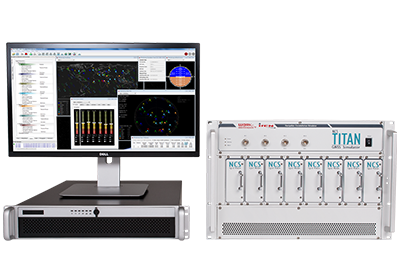
\includegraphics[width=0.48\textwidth]{fig/NCS-Titan_GNSS_Simulator.png}
%\caption{Low-cost ISM Receiver Architecture Scheme}\label{fig:Rx}
\end{wrapfigure}
As a complement, particularly useful in the design phase of the project where methods are adjusted, it is worth mentioning here that have access to a powerful GNSS signal simulator. Namely, the lab I am member of has acquired the NCS Titan GNSS Simulator, the latest product from IFEN. The Titan is a multi-GNSS, multi-frequency and multi-RF output simulator, featuring high fidelity, flexibility and scalability. The available equipment can simulate up to 256 channels and up to 2 RF outputs, generating GPS L1, GPS L5, Galileo E1, and Galileo E5 signals. Among the many characteristics of this high-grade signal simulator, it is of interest here that it is able to incorporate jamming and spoofing attacks, as well as relevant receiver imperfections. This equipment is crucial to test the developed methodologies in a controlled manner, before validation through real data. Additionally, we own USRP and HackRF front-ends which will be used to connect the GNSS Simulator with the GNSS-SDR receiver. This front-ends are a perfect example of the versatile, low-cost hardware components we are interested in this project, featuring a rather poor clock accuracy around $1$ to $20$ ppm depending on the hacks.

% F. Biographical Sketch(es)
% \newsection{D}
\section{Primary Author Biography}

The author of this document and proposed work, Gerald LaMountain, is a first year Communications Control and Signal Processing PhD student in the Electrical and Computer Engineering department at Northeastern University in Boston, Massachusetts. He is advised by Professor Pau Closas, also of Northeastern University and is currently involved in research related to positioning, localization and related applications. Although he has not been previously active in open source software development, his background includes work on distributed single and multiprocessor data processing applications, including software defined radios, through his work at Raytheon BBN Technologies in Cambridge, Massachusetts. This includes collaborative development in C, C++, Python and MATLAB.

% G. Budget Justification
% \newsection{G}
% \input{sections/budget}

%  H. Current and Pending Support
% \newsection{H}
% \input{sections/support}

% I. Facilities, Equipment and Other Resources
% \newsection{I}
% \input{sections/resources}

% J. Special Information and Supplementary Documentation
% \newsection{J}
% \input{sections/data}		% Data Management Plan (Required)

%\input{sections/postdoc} % Postdoctoral Researcher Mentoring Plan (if applicable)

\end{document}
